\documentclass[12pt]{report}

\usepackage[utf8]{inputenc}
\usepackage{stmaryrd}
\usepackage[french]{babel}
\usepackage{amsmath}
\usepackage{graphicx}
\usepackage{subcaption}
\usepackage{color}
\usepackage{amsfonts}

\title{Résolution d'équations différentielles par réseaux de neurones}

\author{
  Matthieu Carreau\\
  Telecom Paris, Institut Polytechnique de Paris\\
  F-91120, Palaiseau, France\\
  \texttt{matthieu.carreau@telecom-paris.fr} \\
  [1em] Supervisors: \\
  Stam Nicolis\\
  Institut Denis Poisson\\
  Université de Tours, Université d'Orléans, CNRS (UMR7013)\\
  Parc de Grandmont, F-37200, Tours, France\\
  \texttt{stam.nicolis@lmpt.univ-tours.fr}\\
  [1em] \\
  Pascal Thibaudeau\\
  CEA Le Ripault\\
  BP 16, F-37260, Monts, France\\
  \texttt{pascal.thibaudeau@cea.fr}
}
\date{Juillet 2022}

\begin{document}

\maketitle

\begin{abstract}
    {\color{red}{Faire un résumé de ce qu'il y a dans ce document}}
\end{abstract}
    
\tableofcontents{}
    
\chapter{Introduction}
\label{Introduction}

{
    \color{red}{Cette partie positionne le travail dans un contexte. Décrire le contexte. Dire ici ce que l'on doit faire et proposer un petit résumé des documents lus de façon à montrer en quoi ils sont pertients pour le problème posé.
    Par exemple : Bidulle et Machin dans la référence~\cite{BiduletMachin2020} ont montré que ... tandis que Truc et Chmuc dans la référence~\cite{TrucetChmuc2020} ont prouvé que...}
    Dans la section~\ref{section_ode_1}, je montrerai que...
    Dans la section~\ref{section_precession}, je montrerai...
    Enfin dans la section~\ref{Conclusion}, je discuterai des résultats obtenus et proposerai quelques perspectives.
}

%%%%%%%%%%%%%%%%%%%%%%%%%%%%%%%%%%%%%%%%%%%%%%%%%%%%%%%%%%%%%%%%%%%%%%%%%%%%%
\chapter{Equation différentielle d'ordre 1}
\label{section_ode_1}

Soit $\Psi$ une fonction réelle à une variable dont la solution satisfait l'équation différentielle suivante, où $\psi_0$ désigne la valeur initiale de la fonction.

\begin{equation}
\left\{
    \begin{aligned}
        \frac{d\Psi(x)}{dx} + \cos(2\pi x) &= 0 \\
        \Psi(0) &= \psi_0
    \end{aligned}
\right.
\label{eq:equa dif}
\end{equation}
On cherche à tester les méthodes présentées dans la section~\ref{Introduction} sur l'équation~(\ref{eq:equa dif}), pour tout $x\in [0,1]$.
L'équation~(\ref{eq:equa dif}) et sa condition initiale donnée en $x=0$, admet une solution analytique unique qui s'écrit
\begin{equation}
    {\Psi}(x) = \psi_0 - \frac{1}{2\pi}\sin(2\pi x)
    \label{eq:solution analytique}
\end{equation}


Cela nous permettra par la suite d'évaluer nos solutions numériques, en les comparant à cette solution analytique.


%%%%%%%%%%%%%%%%%%%%%%%%%%%%%%%%%%%%%%%%%%%%%%%%%%%%%%%%
\section{Solutions en séries de Fourier}

On cherche des solutions numériques approchées de l'équation~(\ref{eq:equa dif}) sous la forme de séries de Fourier tronquées avec $M$ harmoniques.
On écrit pour cela la solution approchée $\Tilde{\Psi}$ comme la somme de deux termes, le premier $\psi_0$ constant non ajustable vérifiant la condition initiale, et 
le deuxième $\mathcal{N}(x,\bf{A})$ dépendant des coefficients $(A_m)_{m\in \llbracket 1,M \rrbracket}$ représentés par le vecteur $\bf{A}$, construit de façon à ne pas influencer la valeur initiale de la fonction.

\begin{equation}
\left\{
    \begin{aligned}
        \Tilde{\Psi}(x) &= \psi_0 + {\mathcal{N}}(x,\bf{A}) \\
        {\mathcal{N}}(x,\bf{A}) &= \sum_{m=1}^{M} A_m \sin(2\pi m x) 
    \end{aligned}
\right.
\label{eq:solution Fourier}
\end{equation}




On définit une fonction d'erreur pour ces solutions potentielles, à partir de la valeur de la dérivée de $\Tilde{\Psi}$ aux $N$ points suivants : $\forall i \in\llbracket 1,N \rrbracket, x_i = \frac{i-1}{N} $

\begin{equation}
    E = \frac{1}{2}\sum_{i=1}^{N}(\sum_{m=1}^{M} 2\pi m A_m \cos(2\pi m x_i)+\cos(2\pi x_i))^2 
\label{eq:fonction d'erreur}
\end{equation}

On cherche à présent le minimum de $E$ en tant que fonction de $\bf{A}$. Une condition nécessaire sur $\bf{A}$ pour être un antécédent d'un minimum
est 
\begin{equation}
    {\forall l \in\llbracket 1,M \rrbracket, \frac{\partial E}{\partial A_l} = 0}
    \label{eq:condition nécessaire A_l}
\end{equation}

Or ces dérivées partielles sont données pour $l \in \llbracket 1,M \rrbracket$ par :

\begin{equation}
    \frac{\partial E}{\partial A_l} = 
    \sum_{i=1}^{N}(\sum_{m=1}^{M} 2\pi m A_m \cos(2\pi m x_i)+\cos(2\pi x_i))
    2\pi l \cos(2\pi l x_i)
\label{eq:gradient}
\end{equation}


Les deux méthodes suivantes ont pour objectif de trouver les coefficients $(A_m)_{m\in \llbracket 1,M \rrbracket}$ qui vérifient la condition \ref{eq:condition nécessaire A_l}, et de vérifier que le vecteur de coefficients
trouvé correspond bien à la solution analytique, i.e $\forall m \in\llbracket 1,M \rrbracket, A_m = -\frac{1}{2\pi}\delta _1 ^m $.


%%%%%%%%%%%%%%%%%%%%%%%%%%%%%%%%%%%%%%%%%%%%%%%%%%%%%%%%
\subsection{Première méthode : inversion d'un système linéaire}

On cherche à résoudre le système linéaire donné par : 
$\displaystyle{\forall l \in\llbracket 1,M \rrbracket, \frac{\partial E}{\partial A_l} = 0}$, on définit pour cela les matrices suivantes :

\begin{equation}
    \mathcal{M} = (r_{m,l})_{(m,l)\in \llbracket 1, M\rrbracket ^2}, 
    \bf{A} = \begin{pmatrix}
                A_1 \\
                A_2 \\
                \vdots \\
                A_M
              \end{pmatrix}, 
    \bf{b} = \begin{pmatrix}
                b_1 \\
                b_2 \\
                \vdots \\
                b_M
              \end{pmatrix}
\label{eq:définition notation}
\end{equation}

\begin{equation}
\forall (m,l) \in \llbracket 1, N\rrbracket ^2,
\left\{
    \begin{aligned}
        r_{m,l} &= 2\pi ml \sum_{i=1}^{N}\cos(2\pi mx_i)\cos(2\pi lx_i) \\
        b_l &= -l\sum_{i=1}^{N}\cos(2\pi x_i)\cos(2\pi lx_i)
    \end{aligned}
\right.
\label{eq:définition coefficients}
\end{equation}

On souhaite alors résoudre le système linéaire en écrivant 
l'équation matricielle le représentant, c'est-à-dire :

\begin{equation}
    \mathcal{M} \bf{A} = \bf{b} \Leftrightarrow \bf{A} = \mathcal{M}^{-1}\bf{b}
\label{eq:équation matricielle}
\end{equation}

On réalise l'implémentation en python, en instanciant 
les matrices définies précédemment et à l'aide de la bibliothèque \emph{numpy}. 
On peut constater que la matrice $\mathcal{M}$ n'est pas toujours inversible
selon le choix de $M$ et $N$. En effet, on peut montrer {\color{red}(à rajouter en annexe)} que c'est nécessairement le cas lorsque $M>N$, 
mais on remarque également qu'elle ne l'est pas non plus lorsque $M$ et $N$ sont proches par exemple pour $M=N=10$. Il serait interressant d'approfondir ce point
pour savoir si cela se traduit par le fait que $E$ admette plusieurs minimums locaux par exemple.
Il semble que choisir $N\gg M$ soit suffisant pour que $\mathcal{M}$ soit inversible. On choisira alors $M=10, N=100$ pour la suite.
On obtient alors les coefficients présentés en figure \ref{fig:résultats 1 inv} avec les valeurs absolues des erreurs de chacun par rapport à la valeur théorique. 
On constate que les erreurs sur chaque coefficient
est inférieure à $10^{-16}$, on valide donc cette première méthode.


\begin{figure}
    \centering
    \begin{subfigure}[b]{0.4\textwidth}
        \centering
        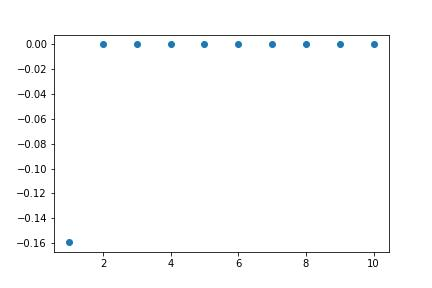
\includegraphics[width=0.9\textwidth, height=0.9\textwidth]{coefs_1_inv.jpg}
        \caption{Coefficients trouvés}
    \end{subfigure}
    \hfill
    \begin{subfigure}[b]{0.4\textwidth}
        \centering
        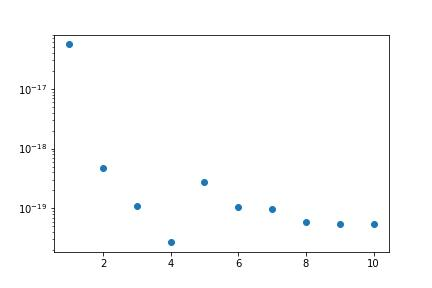
\includegraphics[width=0.9\textwidth, height=0.9\textwidth]{coefs_1_inv_erreur.jpg}
        \caption{Valeurs absolue de l'erreur pour chaque coefficient}
    \end{subfigure}
       \caption{Résultats de la méthode de l'inversion de système}
       \label{fig:résultats 1 inv}
\end{figure}



%%%%%%%%%%%%%%%%%%%%%%%%%%%%%%%%%%%%%%%%%%%%%%%%%%%%%%
\subsection{Seconde méthode : descente de gradients}

On définit les paramètres suivants :

\begin{equation}
    \alpha>0, 
    \bf{A}^{(0)} = \begin{pmatrix}
                A_1^{(0)} \\
                A_2^{(0)} \\
                \vdots \\
                A_M^{(0)}
              \end{pmatrix},
    \bf{g}^{(0)} = \begin{pmatrix}
                \frac{\partial E^{(0)}}{\partial A_1^{(0)}} \\
                \frac{\partial E^{(0)}}{\partial A_2^{(0)}} \\
                \vdots \\
                \frac{\partial E^{(0)}}{\partial A_M^{(0)}}
              \end{pmatrix},     
\label{eq:définition descente de gradients}
\end{equation}

Puis on calcule itérativement :

\begin{equation}
    \bf{A}^{(k+1)} = \bf{A}^{(k)} - \alpha\bf{g}^{(k)} 
\label{eq:équation récurrence descente gradients}
\end{equation}

On cherche à trouver le coefficient $\alpha$ optimal qui assure la convergence tout en maximisant la vitesse de convergence.
On exprime tout d'abord le gradient en fonction de la matrice $\mathcal{M}$ et du vecteur $\bf{b}$ définis précédemment qui sont indépendants de $\bf{A}$ et de $k$:
\begin{equation}
    \bf{g}^{(k)} = \mathcal{M}\bf{A}^{(k)} - \bf{b}
\label{eq:expression matricielle gradient}
\end{equation}

Ainsi, l'équation de récurrence (\ref{eq:équation récurrence descente gradients}) se réécrit comme une suite arithmético-géométrique de vecteurs :

\begin{equation}
    \bf{A}^{(k+1)} = (\mathcal{I}_M - \alpha \mathcal{M} )  \bf{A}^{(k)} + \alpha\bf{b}
\label{eq:équation récurrence descente gradients v2}
\end{equation}

On en déduit que la suite converge si et seulement si la norme $(\mathcal{R}_\alpha ^n)_{n\in \mathbb{N}}$ tend vers 0de le maximum du module des valeurs propres de la matrice
$\mathcal{R}_\alpha = \mathcal{I}_M - \alpha \mathcal{M}$ est strictement inférieur à 1. De plus, elle convergera
d'autant plus vit que ce maximum est faible.
On trace donc ce maximum en fonction de $\alpha$ en figure \ref{fig:choix alpha 1D}. 
On en déduit la valeur critique $\alpha_c = 6.2807.10^{-5}$, pour laquelle le maximum des modules vaut $1$, ainsi que la 
valeur $\alpha_{min} = 6.2189.10^{-5}$ pour laquelle le maximum des modules est minimum.

On éxécute l'algorithme en parallèle pour les deux valeurs de $\alpha$ trouvées précédemment ainsi que pour une valeur 
$\alpha_1 = 6.3.10^{-5}$, tel que le maximum des modules des valeurs propres de $\mathcal{R}_\alpha$ soit supérieur à 1.
On montre l'évolution de l'erreur en fonction du nombre d'itérations en figure \ref{fig:erreur selon alpha}. On constate 
que $\alpha_{min}$ donne lieu à une décroissance exponentielle de l'erreur pendant les 2000 premières itérations, qui 
devient ensuite stationnaire. Tandis que $\alpha_1$ donne une erreur qui croît exponentiellement car la norme de 
$(\mathcal{R}_\alpha ^n)_{n\in \mathbb{N}}$ diverge exponentiellement. La valeur $\alpha_c$ donne une erreur constante, 
elle correspond au cas limite entre les 2 cas précédents.

\begin{figure}
    \centering
    \begin{subfigure}[b]{0.4\textwidth}
        \centering
        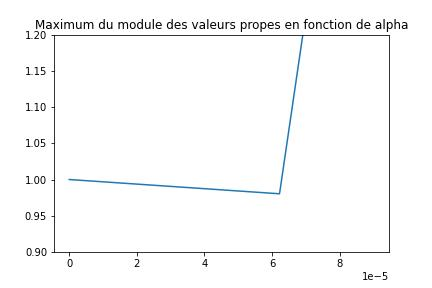
\includegraphics[width=0.8\textwidth, height=0.8\textwidth]{choix_alpha_1D.jpg}
        \caption{$\alpha \in [0, 10^{-4}]$}
    \end{subfigure}
    \hfill
    \begin{subfigure}[b]{0.4\textwidth}
        \centering
        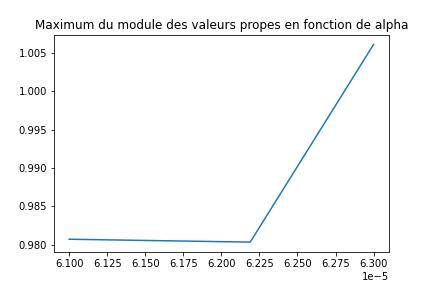
\includegraphics[width=0.8\textwidth, height=0.8\textwidth]{choix_alpha_1D_zoom.jpg}
        \caption{Au voisinage de l'intersection avec 1}
    \end{subfigure}
       \caption{Maximum des valeurs propres de $\mathcal{R}_\alpha$ en fonction de $\alpha$}
       \label{fig:choix alpha 1D}
\end{figure}


\begin{figure}
    \centering
    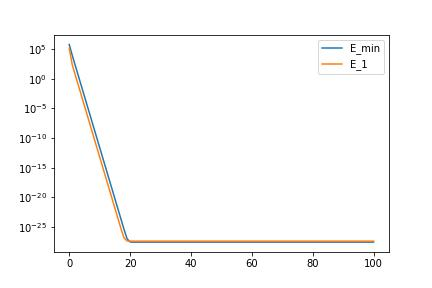
\includegraphics[width=0.8\textwidth]{comparaison_erreurs_selon_alpha_1D.jpg}
    \caption{Erreurs en fonction du nombre d'itérations pour 3 valeurs de $\alpha$}
    \label{fig:erreur selon alpha}
    \end{figure}


On retient donc les résultats obtenus pour $\alpha_{min}$ que l'on montre en figure
 \ref{fig:résultats 1 DG} avec les valeurs absolues des erreurs de chacun par rapport à la valeur théorique. 
On constate que les erreurs sur chaque coefficient
est inférieure à $10^{-16}$, on valide donc cette seconde méthode.


\begin{figure}
    \centering
    \begin{subfigure}[b]{0.4\textwidth}
        \centering
        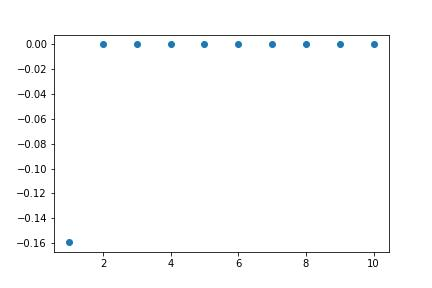
\includegraphics[width=0.9\textwidth, height=0.9\textwidth]{coefs_1_DG.jpg}
        \caption{Coefficients trouvés}
    \end{subfigure}
    \hfill
    \begin{subfigure}[b]{0.4\textwidth}
        \centering
        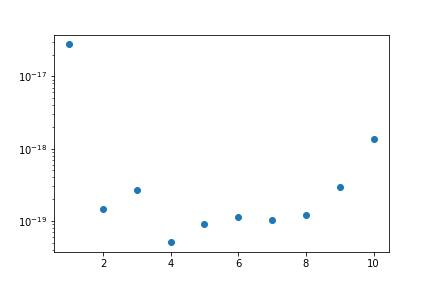
\includegraphics[width=0.9\textwidth, height=0.9\textwidth]{coefs_1_DG_erreur.jpg}
        \caption{Valeurs absolue de l'erreur pour chaque coefficient}
    \end{subfigure}
       \caption{Résultats de la méthode de descnte de gradients}
       \label{fig:résultats 1 DG}
\end{figure}



%%%%%%%%%%%%%%%%%%%%%%%%%%%%%%%%%%%%%%%%%%%%%%%%%%%%%%%%%%%%%%%%%%%%
\section{Solutions par réseau de neurones}

On cherche à présent à utiliser un réseau de neurones pour approcher la solution de l'équation différentielle. On cherche désormais des solutions approchées sous la forme suivante :

\begin{equation}
\left\{
    \begin{aligned}
        \Tilde{\Psi}(x) &= \psi_0 + {\mathcal{N}}(x,P) \\
        {\mathcal{N}}(x,P) &= \sum_{j=1}^{H} v_j \sigma(w_jx+b_j)
    \end{aligned}
\right.
\label{eq:solution NN}
\end{equation}

${\mathcal{N}}(x,P)$ correspond donc à la sortie d'un réseau de neurones dont l'architecture est présentée en figure \ref{fig:NN}, contenant une couche cachée intermédiaire, qui réalise en sortie une somme pondérée de sigmoïdes, la fonction utilisée est ${\displaystyle{\forall x \in \mathbf{R}, \sigma(x) = \frac{1}{1+e^{-x}}}}$. Les paramètres $P$ à ajuster sont désormais les coefficients $(w_j)_{j\in \llbracket 1,H \rrbracket}$, $(b_j)_{j\in \llbracket 1,H \rrbracket}$ et $(v_j)_{j\in \llbracket 1,H \rrbracket}$.

{\color{red}Peux-tu donner une référence pour quelqu'un qui cherche ce que tout ceci veut dire?}
\begin{figure}
\centering
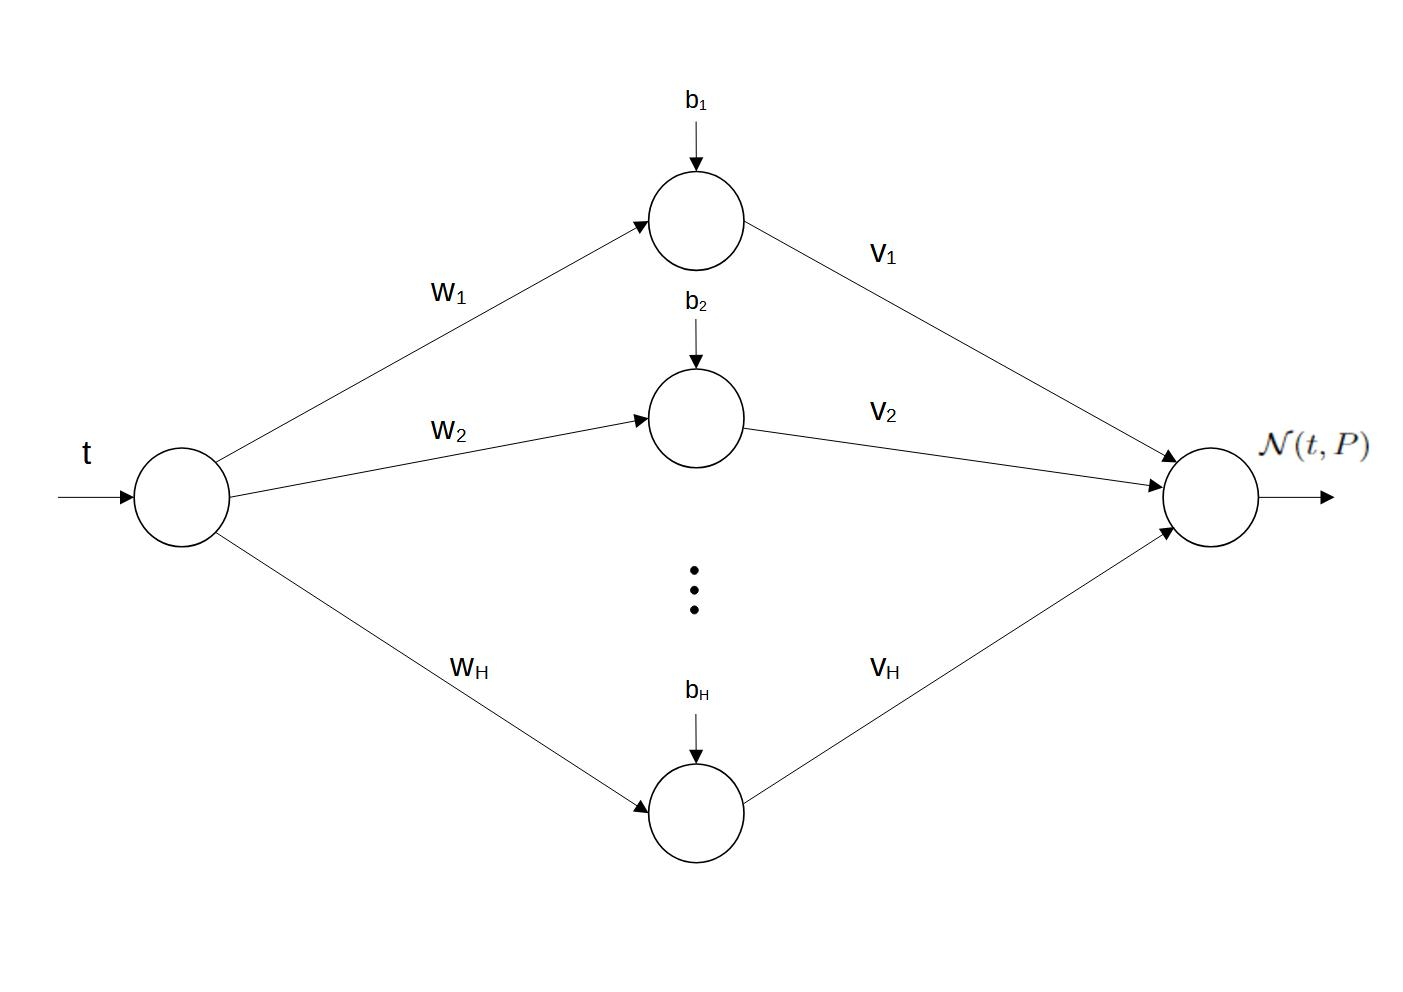
\includegraphics[width=0.8\textwidth]{NN.jpg}
\caption{\label{fig:NN}Réseau de neurones}
\end{figure}

On définit une nouvelle fonction d'erreur, calculée à partir des $N$ points suivants : $\forall i \in\llbracket 1,N \rrbracket, x_i = \frac{i-1}{N-1} $ 
%(Contrairement à la fonction d'erreur définie pour les solutions en série de Fourier, 
%on définit ici les points de tests de façon à inclure $x_N = 1$ car la fonction définie n'est plus nécessairement périodique, alors que ce point aurait été redondant avec le point $x_0 = 0$ pour les fonctions 1\_périodiques)

\begin{equation}
        E(P) = \sum_{i=1}^{N} (\frac{d\Tilde{\Psi}}{dx}(x_i) + \cos(2\pi x_i))^2
\label{eq:erreur NN}
\end{equation}
{\color{red}L'équation~(\ref{eq:erreur NN}) est-elle correcte ?}

On calcule ensuite les expressions analytiques des dérivées partielles de $E(P)$ par rapport à chaque paramètre ajustable, puis on cherche à minimiser cette erreur à l'aide de l'algorithme de descente de gradients.

%%%%%%%%%%%%%%%%%%%%%%%%%%%%%%%%%%%%%%%%%%%%%%%%%%%%%%
\subsection{Résultats obtenus}
On initialise l'algorithme avec les paramètres suivants :
$(H=4, N=20)$
On obtient une erreur de $1,2.10^{-2}$ et une estimation visible en figure \ref{fig:resultat_NN}. Cela permet de valider notre modèle sur l'étude à une dimension.

\begin{figure}
\centering
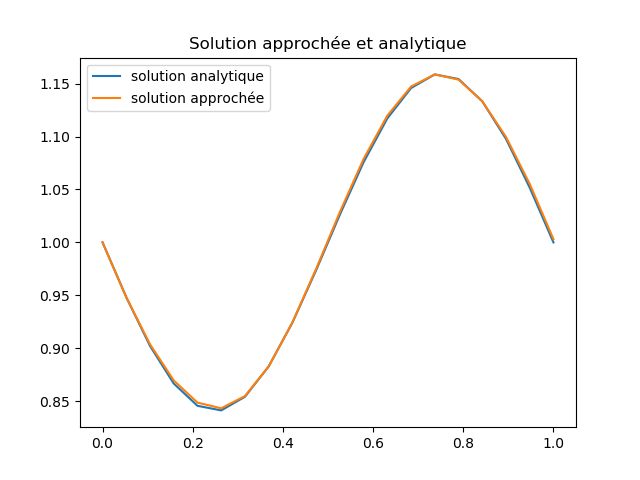
\includegraphics[width=0.8\textwidth]{resultat_NN.png}
\caption{\label{fig:resultat_NN}estimation de la solution par un réseau de neurones}
\end{figure}

%%%%%%%%%%%%%%%%%%%%%%%%%%%%%%%%%%%%%%%%%%%%%%%%%%%%%%
\chapter{Mouvement de précession}
\label{section_precession}
On s'intéresse désormais au problème de la précession d'un moment magnétique dans un champ magnétique constant. On le modélise par les équations suivantes pour $t\in [0,1]$ :

\begin{equation}
\left\{
    \begin{aligned}
        \frac{dv_x}{dt} &= \omega v_y \\
        \frac{dv_y}{dt} &= -\omega v_x
    \end{aligned}
\right.
\end{equation}
avec les conditions initiales
\begin{equation}
\left\{
    \begin{aligned}
        v_x(0) &= V_0 \\
        v_y(0) &= 0
    \end{aligned}
\right.
\label{eq:équations couplées}
\end{equation}
dont la solution analytique vaut
\begin{equation}
\left\{
    \begin{aligned}
        v_x(t) &=  V_0 \cos(2\omega t)\\
        v_y(t) &= -V_0 \sin(2\omega t)
    \end{aligned}
\right.
\label{eq:solution analytique couplée}
\end{equation}

\section{Solutions en séries de Fourier}
On cherche des solutions numériques approchées sous la forme de séries de Fourier tronquées avec $M$ harmoniques, en posant la forme suivante :

\begin{equation}
\left\{
    \begin{aligned}
        \Tilde{v}_x(t) = V_0 + \sum_{m=1}^{M} A_m (\cos(m\omega t)-1) + B_m \sin(m\omega t) \\
        \Tilde{v}_y(t) = \sum_{m=1}^{M} -A_m \sin(m\omega t) + B_m (\cos(m\omega t)-1)
    \end{aligned}
\right.
\label{eq:solution Fourier couplée}
\end{equation}

Les coefficients $(A_m)_{m\in \llbracket 1,M \rrbracket}$ et $(B_m)_{m\in \llbracket 0,M \rrbracket}$ sont les paramètres à ajuster.
On cherche à obtenir la solution analytique, i.e $\forall m \in\llbracket 0,M \rrbracket, A_m = \delta _1 ^m $ et $\forall m \in\llbracket 1,M \rrbracket, B_m = 0 $. On remarque que le coefficient $A_0$ n'a aucune influence.

On définit une fonction d'erreur pour ces solutions potentielles, en s'interressant aux $N$ points suivants : $\forall i \in\llbracket 1,N \rrbracket, t_i = \frac{i-1}{N} $ :

\begin{equation}
        E(P) = \sum_{i=1}^{N} (\frac{d\Tilde{v}_x}{dt}(t_i) - \omega \Tilde{v}_y(t_i))^2 + (\frac{d\Tilde{v}_y}{dt}(t_i) + \omega \Tilde{v}_x(t_i))^2
\label{eq:erreur descente gradient couplées}
\end{equation}

On utilise ensuite la méthode de descente de gradients définie précédemment, en calculant les dérivées partielles suivantes :
$(\frac{\partial E}{\partial A_l}, \frac{\partial E}{\partial B_l})_{l \in \llbracket 1,M \rrbracket}$

On peut se ramener à l'écriture du cas à une dimension définissant le vecteur $\bf{P}$ comme la concaténation des 
vecteurs $\bf{A}$ et $\bf{B}$ et le vecteur $\bf{g}$ comme le vecteur contenant les dérivées  partielles de $E$
par rapport à chaque composante de $\bf{P}$. 

\begin{equation}
    \bf{P}^{(k)} = \begin{pmatrix}
                A_1^{(k)} \\
                \vdots \\
                A_M^{(k)} \\
                B_1^{(k)} \\
                \vdots \\
                B_M^{(k)}
              \end{pmatrix},
    \bf{g}^{(k)} = \begin{pmatrix}
                \frac{\partial E^{(k)}}{\partial A_1^{(k)}} \\
                \vdots \\
                \frac{\partial E^{(k)}}{\partial A_M^{(k)}} \\
                \frac{\partial E^{(k)}}{\partial B_1^{(k)}} \\
                \vdots \\
                \frac{\partial E^{(k)}}{\partial B_M^{(k)}} 
              \end{pmatrix},     
\label{eq:définition descente de gradients 2D}
\end{equation}

Il existe alors une nouvelle matrice $\mathcal{M}$ d'ordre $2M$ ainsi qu'un nouveau vecteur $\bf{b}$ de taille $2M$ tels que les 
équations définissant la descente de gradients soient les suivantes :

\begin{equation}
    \bf{P}^{(k+1)} = \bf{P}^{(k)} - \alpha\bf{g}^{(k)} 
\label{eq:équation récurrence descente gradients 2D}
\end{equation}

\begin{equation}
    \bf{g}^{(k)} = \mathcal{M}\bf{P}^{(k)} - \bf{b}
\label{eq:expression matricielle gradient 2D}
\end{equation}

\begin{equation}
    \bf{P}^{(k+1)} = (\mathcal{I}_M - \alpha \mathcal{M} )  \bf{P}^{(k)} + \alpha\bf{b}
\label{eq:équation récurrence descente gradients v2 2D}
\end{equation}

On réalise la même étude qu'en dimension 1 pour la recherche du coefficient $\alpha_{min}$ qui minimise le maximum
des modules des valeurs propres de $\mathcal{R}_\alpha = \mathcal{I}_M - \alpha \mathcal{M}$, ainsi que le coefficient 
$\alpha_c$ à ne pas dépasser, à partir duquel ce maximum et supérieur à 1 et la suite diverge.
On trouve les valeurs suivantes $\alpha_{min} = 6.0906.10^{-6}$ et $\alpha_c = 6.1146.10^{-6}$,  et l'évolution du 
maximum en fonction de alpha est montré en figure \ref{fig:choix_alpha_2D}.


\begin{figure}
    \centering
    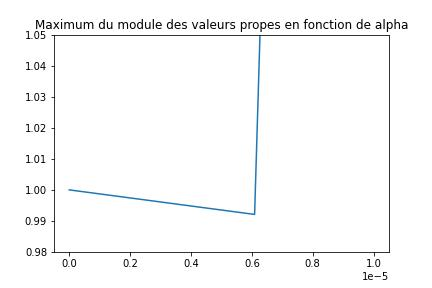
\includegraphics[width=0.7\textwidth]{choix_alpha_2D.jpg}
    \caption{\label{fig:choix_alpha_2D}Evolution du maximum du module en fonction de $\alpha$}
\end{figure}

On éxécute l'algorithme en choisissant la valeur $\alpha_{min}$ précédente et on montre l'évolution de 
l'erreur en fonction du nombre d'itérations en figure \ref{fig:Erreur_2_DG}. 
On constate comme dans le cas à 1 dimension que $\alpha_{min}$ donne lieu à une décroissance exponentielle de l'erreur, 
cette fois pendant les 4500 premières itérations, qui devient ensuite quasiment stationnaire, de l'ordre de $10^{-25}$.

\begin{figure}
    \centering
    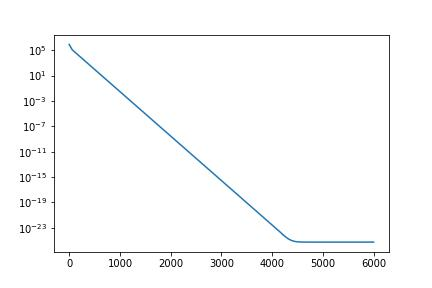
\includegraphics[width=0.7\textwidth]{Erreur_2_DG.jpg}
    \caption{\label{fig:Erreur_2_DG}Valeur de la fonction d'erreur en fonction du nombre d'itérations}
\end{figure}

Les coefficients finaux de $P$ ainsi que les valeurs absolues de leurs erreurs sont représentées 
en figure \ref{fig:résultats 2 DG}.
On peut constater que l'on retrouve bien les coefficients attendus, avec une erreur au maximum de 
l'ordre de $10^{-15}$.

\begin{figure}
    \centering
    \begin{subfigure}[b]{0.4\textwidth}
        \centering
        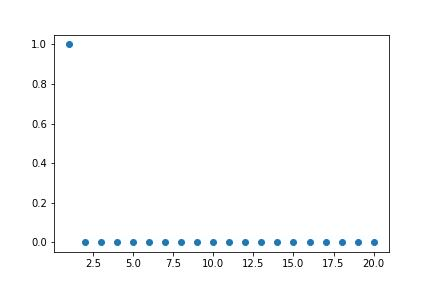
\includegraphics[width=0.9\textwidth, height=0.9\textwidth]{coefs_2_DG.jpg}
        \caption{Coefficients trouvés}
    \end{subfigure}
    \hfill
    \begin{subfigure}[b]{0.4\textwidth}
        \centering
        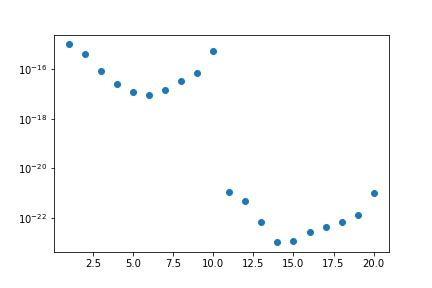
\includegraphics[width=0.9\textwidth, height=0.9\textwidth]{coefs_2_DG_erreur.jpg}
        \caption{Valeurs absolue de l'erreur pour chaque coefficient}
    \end{subfigure}
       \caption{Résultats de la méthode de descente de gradients pour le mouvement de précession}
       \label{fig:résultats 2 DG}
\end{figure}


\chapter{Conclusion et perspectives}
\label{Conclusion}

\begin{thebibliography}{2}
    \bibitem{BiduletMachin2020}{C.Bidule and A.Machin, Journal of Computer Power {\bf 12} 123 (2020)}
    \bibitem{TrucetChmuc2020}{C.Truc and T.Chmuc, (2020)}
\end{thebibliography}


\end{document}

